\documentclass[]{report}
\usepackage[hmargin=1.25in,vmargin=1in]{geometry} %调整页边距
% \usepackage[inner=1in,outer=1.25in]{geometry} %书籍左右不等宽排版
\usepackage[utf8]{inputenc}
\usepackage[]{ctex} %据说可以直接调用诸如 \kaishu \fangsong \heiti 的命令修改字体
\usepackage[svgnames]{xcolor} % Using colors
% \usepackage{background} % To include background images
\usepackage{fancyhdr} % Needed to define custom headers/footers
\usepackage[]{xeCJK}
\setCJKmainfont[BoldFont = STHeiti, ItalicFont = STKaiti]{Songti SC Light} %中文主字体
\setCJKsansfont[BoldFont = Weibei SC, ItalicFont = HanziPen SC]{Xingkai SC Light} %中文无衬线字体
\setCJKmonofont[BoldFont = Libian SC, ItalicFont = STFangsong]{Yuanti SC Light} %中文等宽字体
\setmainfont{Times New Roman} %\rmfamily
\setsansfont[ItalicFont = American Typewriter]{Comic Sans MS} %\sffamily
\setmonofont{Courier} %\ttfamily
\newfontfamily\monaco{Courier}
\usepackage{titlesec}
\titleformat{\chapter}{\centering\huge\bfseries}{第~\thechapter~章}{1em}{}

\usepackage{ulem} %解决下划线、删除线之类的
\usepackage{listings}
\lstset{
language=C++,
numberstyle = \monaco\color[HTML]{FFD700},
basicstyle = \monaco,
keywordstyle = \color{blue}\bfseries,
commentstyle=\color[HTML]{006400}, %DarkGreen
tabsize = 4,
%backgroundcolor=\color{bg}
emph = {int,float,double,char,void},emphstyle=\color[HTML]{800080}, % Purple
emph ={[2]const, typedef},emphstyle = {[2]\color[HTML]{4682B4}} %SteelBlue
}

\usepackage{amsmath} %数学公式问题
\usepackage{amsthm} %公式环境,如proof
\usepackage{booktabs} %三线表
\newcommand{\tabincell}[2]{\begin{tabular}{@{}#1@{}}#2\end{tabular}} %解决单元格内部换行的问题
% 比如这个 Beijing & 0,5 & 1,6 & 2,7 & 3,8 & 4,9 & The number changes every 3 months \\
% 改成这个 \tabincell{l}{Beijing}& \tabincell{c}{0,5}& \tabincell{c}{1,6}& \tabincell{c}{2,7}& \tabincell{c}{3,8}& \tabincell{c}{4,9}& \tabincell{c}{The number changes \\ every 3 months} \\
% 一个单元格过长,整行都需要修改
% 可以配合 \resizebox*{h-width}{v-width}{contents, e.g.tabular} 使用

\usepackage{mathrsfs} %在公式里面使用那个最花的字体
\usepackage{amssymb} %公式里面用空心黑体和旧式字体
\usepackage{amssymb} %AMS符号
\usepackage{amsthm} %AMS定理环境

\usepackage{markdown} %使用markdown语法,在编译时需要打开 shell-escape 标记,即 $ xelatex --shell-escape example.tex
\markdownSetup{hashEnumerators = true} %允许使用 #. 的方式编写有序列表
\markdownSetup{inlineFootnotes = true} %允许使用脚注形式的超链接,调用语法为 [anchor](uri), ^[footnote], <uri>
\markdownSetup{fencedCode = true} %以反引号和缩进来插入代码段,相当于 verbatim
\markdownSetup{
  pipeTables = true
} %支持表格的用法 (图片已经在markdown包里面支持了)
% \usepackage{booktabs} %解决三线表的线条粗细问题

\usepackage{graphicx} %插入图片
\usepackage{pdfpages} %插入PDF文件
\usepackage{makeidx}

\usepackage{tikz} %带圈字符
\usepackage{etoolbox} %带圈字符 (提供robustify)
\usepackage{enumitem}
\newcommand*{\circled}[1]{\lower.7ex\hbox{\tikz\draw (0pt, 0pt)%
    circle (.5em) node {\makebox[1em][c]{\small #1}};}} %新定义命令:带圈字符
\robustify{\circled}
% \usepackage{enumerate} %有序列表

\usepackage{hyperref} %超链接
% \usepackage[hidelinks]{hyperref} %隐藏超链接的红框
\markdownSetup{
  inlineFootnotes = true,
  renderers = {
    link = {\href{#3}{#1}},
  }
} % markdown块中使用直接点进去的超链接
% \setlist[enumerate,1]{label=(\arabic*).,font=\textup,leftmargin=7mm,labelsep=1.5mm,topsep=0mm,itemsep=-0.8mm}
% \setlist[enumerate,2]{label=(\alph*).,font=\textup,leftmargin=7mm,labelsep=1.5mm,topsep=-0.8mm,itemsep=-0.8mm}

\usepackage{braket}

%%%%%% Setting up the style

% \setlength\parindent{0pt} % Gets rid of all indentation
% \backgroundsetup{contents={\includegraphics[width=\textwidth]{ustc-name.pdf}},scale=0.4,placement=top,opacity=0.6,color=cyan,vshift=-20pt} %  USTC Logo

\pagestyle{fancy} % Enables the custom headers/footers

% Use Default Headers
% \lhead{} \rhead{} % Headers - all  empty

% \title{\vspace{-1.8cm}  \color{DarkRed} Laboratory Rotation Report}
% \subtitle{Title of the proposal % Title of the rotation project
% \vspace{-2cm} }
% \date{\today} % No date

\lfoot{\color{Grey} \textit{上官凝}}  % Write your name here
\rfoot{ \color{Grey} 程序设计II复习笔记 }
\cfoot{\color{Grey} \thepage}

\renewcommand{\headrulewidth}{0.0pt} % No header rule
\renewcommand{\footrulewidth}{0.4pt} % Thin footer rule

\title{\Huge \color{DarkRed} 程序设计笔记}
\author{\textit{上官凝}}
\date{\today}

\linespread{1.3} %行间距为1.3倍默认间距 (1.3 x 1.2倍字符宽度)

\makeindex

\begin{document}
\theoremstyle{definition} \newtheorem{theorem}{Thm}[section] %定义一个定理Thm,序号为section的下一级序号
\theoremstyle{definition} \newtheorem{definition}{Def}[section] %定义一个定义Def,序号为section的下一级序号
\theoremstyle{plain} \newtheorem{lemma}{lemma}[section] %引理

	\maketitle
	\newpage

	\tableofcontents
	\newpage

	\chapter{C语言进阶、巩固和补充}
	\section{输入输出}
		\paragraph{\texttt{scanf()}} 第一个参数是格式字符串,后面的参数是变量的地址,函数作用是按照第一个参数指定的格式,将数据读入后面的变量。返回值:
		\begin{enumerate}
			\item \verb|>0|:成功读入的数据项个数
			\item \verb|0|:没有项被赋值
			\item \verb|EOF|:第一个尝试输入的字符是EOF(结束)
		\end{enumerate}
		\paragraph{\texttt{printf()}} 第一个参数是格式字符串,后面的参数是待输出的变量,函数作用是按照第一个参数指定的格式,将后面的变量在屏幕上输出。返回值:
		\begin{enumerate}
			\item $\ge0$:成功打印的字符数
			\item $<0$:出错
		\end{enumerate}
		\paragraph{格式字符串的格式控制符号}如下表所示
		\begin{table}[h]
			\centering
			\caption{格式控制符号}
			\begin{tabular}{c|c}
				\toprule
				符号&含义\\
				\midrule
				\% d&读入或输出 \verb|int|变量\\
				\% c&读入或输出 \verb|char|变量\\
				\% f&读入或输出 \verb|float|变量\\
				\% s&读入或输出 \verb|char *| 变量\\
				\% lf&读入或输出 \verb|double| 变量\\
				\% e&以科学计数法格式输出数值\\
				\% x&以十六进制读入或输出 \verb|int| 变量\\
				\% p&输出指针地址值  \\
				\% .5lf&输出浮点数,精确到小数点后5位\\
				\bottomrule
			\end{tabular}
		\end{table}
	\section{函数指针}
		\href{https://en.wikipedia.org/wiki/Function_pointer}{函数指针}可以像一般函数一样,用于调用函数、传递参数。在如 C 这样的语言中,通过提供一个简单的选取、执行函数的方法,函数指针可以简化代码。函数指针只能指向具有特定特征的函数。因而所有被同一指针运用的函数必须具有相同的参数和返回类型。与引用数据值相反,函数指针指向内存中的可执行代码。因为指向函数的指针实际上包含了函数的入口点的内存地址,所以赋给指针变量的地址就是函数的入口地址,从而该指针就可以用来代替函数名。这一特性也使得函数指针可以作为参数传递给其他函数。由此可见,可以定义一个指向函数的指针变量,它可以被处理,如传递给函数,或放置在数组中等等。
		\subsection{函数指针的定义}
		定义一个函数指针,基本格式与定义一个普通指针类似。\par
		普通指针的声明:\verb|int *pa;|\qquad 函数指针的声明:\verb|double (*func1)(double);|\par
		普通指针的赋值:\verb|int *pa = &a;|\par 函数指针的赋值:\verb|double (*func1)(double) = myfunc;|,在这里,\verb|myfunc|是另外定义的一个函数 \verb|double myfunc(double x);|,需要在函数指针使用之前预先声明或定义。\par
		应注意的是,函数名本身也是一个const指针,正如一个数据变量的\& a一样,所以在使用的时候也可以直接将函数名传递给调用者函数
		\subsection{函数指针的应用}
		常见的函数指针的应用是\verb|qsort()|(快排函数)
		\begin{figure}[h]
			\centering
			\begin{minipage}{18em}
				\centering
				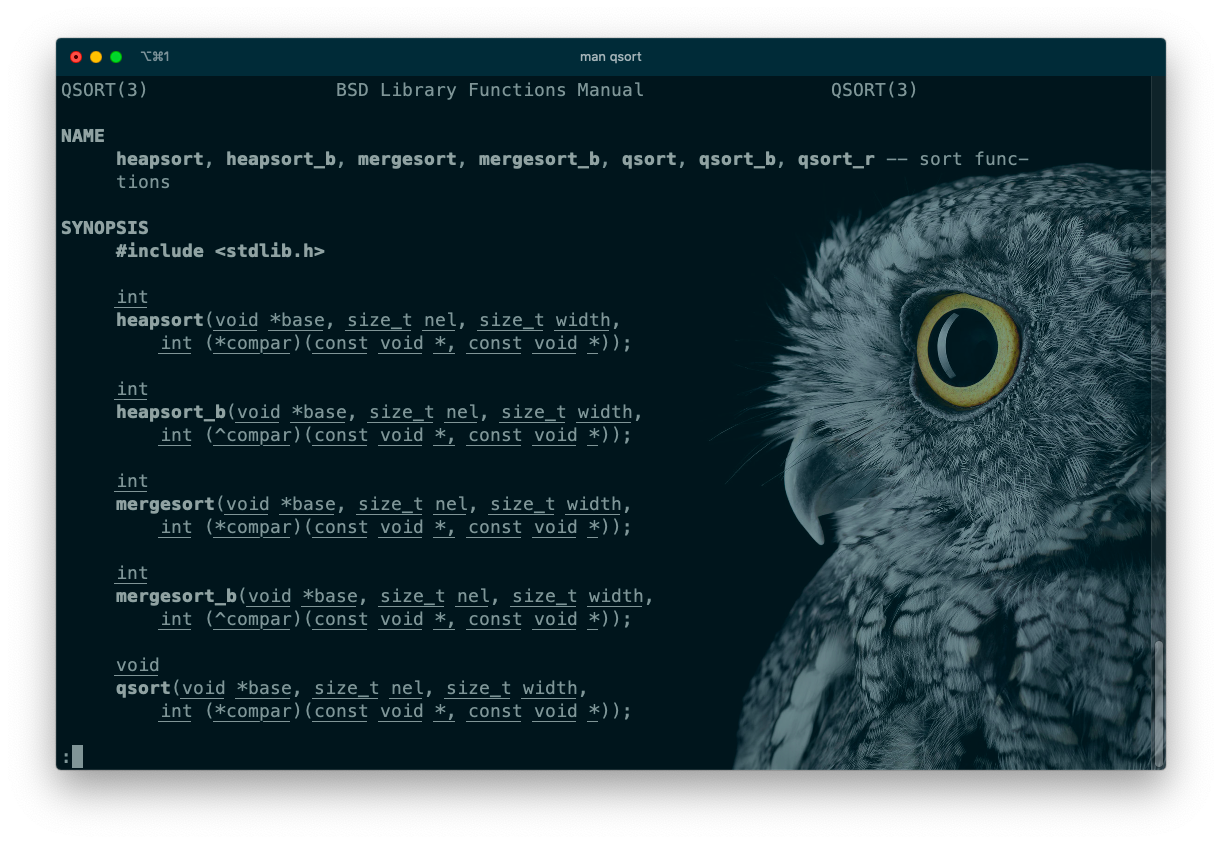
\includegraphics[scale = 0.15]{images/qsort_family.png}
				\caption{\texttt{qsort()} Family}
			\end{minipage}
			\quad
			\begin{minipage}{18em}
				\centering
				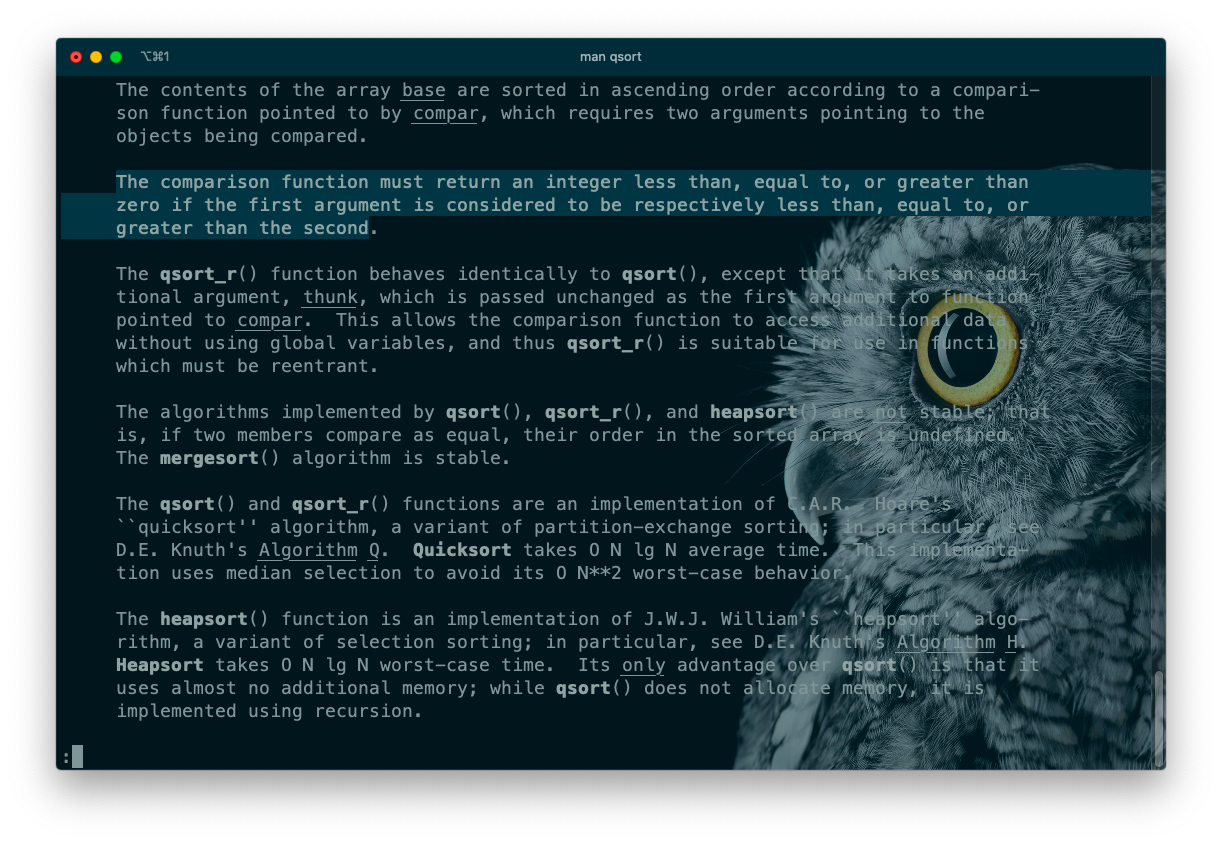
\includegraphics[scale = 0.15]{images/qsort_discription.png}
				\caption{Usage Description}
			\end{minipage}
		\end{figure}
		排序就是一个不断比较并交换位置的过程。\verb|qsort()|如何在连元素的类型是什么都不知道的情况下,比较两个元素并判断哪个应该在前呢?答案是,\verb|qsort()|函数在执行期间,会通过\verb|compar|指针调用 “比较函数”,调用时将要比较的两个元素的地址传给“比较函数”,然后根据“比较函数”返回值判断两个元素哪个更应该排在前面。这个“比较函数”不是C/C++的库函数,而是由使用\verb|qsort()|的程序员编写的。在调用\verb|qsort()|时,将“比较函数”的名字作为实参传递给\verb|compar|。程序员当然清楚该按什么规则决定哪个元素应该在前,哪个元素应该在后,这个规则就体现在“比较函数”中。\par
		比如下面这个简单的\href{https://blog.csdn.net/weixin_45494811/article/details/104471520}{例子}
		\begin{table}
			\centering
			\begin{lstlisting}
typedef struct
{
	int number;
	int score;
} stu;

int self_cmp(const void * a, const void * b)
{
	stu * _a = (stu *) a;
	stu * _b = (stu *) b;
	if (*_a->score != *_b->score)
	{
		return *_b->score - *_a->score; // 从大到小排序
	}
	else
		return *_a->number - *_b->number;
}
// 在主函数中调用qsort(array, array_lenth, sizeof(stu), self_cmp);
// 这样就是先按照成绩降序排列,成绩相等时按照编号升序排列
			\end{lstlisting}
		\end{table}
		\section{动态内存分配}
		众所周知,在经典C语言中,使用\verb|malloc()|函数来进行堆空间分配。而C++提供了\verb|new|\textbf{运算符}来处理这个事情。\verb|new|运算符可以分配一个数据,或者一个数组。此表达式也具有返回值,即若返回值为NULL,则空间分配失败\textsf{\textit{(不是说lazy策略,不使用就不实际分配吗\dots?)}}。配合\verb|delete()|使用,否则会造成内存空间泄漏
	\section{命令行参数}
		主函数新写法:
		\begin{lstlisting}
			int main(int argc, char *argv[]);
		\end{lstlisting}
		可以参考一下\href{https://blog.csdn.net/weixin_43815930/article/details/88558991}{这篇文章}。
	\section{一些库函数}
		\subsection{数学函数}
		在\verb|math.h|中声明
		\begin{table}[h]
			\centering
			\caption{常用的数学函数}
			\begin{tabular}{c|c}
				\toprule
				函数&功能\\
				\midrule
				abs(x)&求整型数x的绝对值\\
				cos(x)&求x(弧度)的余弦\\
				fabs(x)&求浮点数x的绝对值\\
				ceil(x)&求不小于x的最小整数\\
				floor(x)&求不大于x的最小整数\\
				log(x)&求x的自然对数\\
				log10(x)&求x的对数(底为10)\\
				pow(x,y)&求x的y次方\\
				sin(x)&求x(弧度)的正弦\\
				sqrt(x)&求x的平方根\\
				\bottomrule
			\end{tabular}
		\end{table}
		\subsection{字符处理函数}
		在\verb|ctype.h|中声明
		\begin{table}[h]
			\centering
			\caption{字符处理函数}
			\begin{tabular}{c|c}
				\toprule
				函数&功能\\
				\midrule
				int isdigit(int c)&判断c是否是数字字符\\
				int isalpha(int c)&判断c 是否是一个字母\\
				int isalnum(int c)&判断c是否是一个数字或字母\\
				int islower(int c)&判断 c 是否是一个小写字母\\
				int islower(int c)&判断 c 是否是一个小写字母\\
				int isupper(int c)&判断 c 是否是一个大写字母\\
				int toupper(int c)&如果 c 是一个小写字母,则返回其大写字母\\
				int tolower(int c)&如果 c 是一个大写字母,则返回其小写字母\\
				\bottomrule
			\end{tabular}
		\end{table}
		\subsection{字符串和内存操作函数}
		在\verb|string.h|中声明
		\begin{table}[h]
			\centering
			\caption{字符串和内存操作函数}
			\resizebox*{\textwidth}{33em}{
			\begin{tabular}{c|c}
				\toprule
				函数&功能\\
				\midrule
				\tabincell{c}{char * strchr(char * s, int c)}&\tabincell{c}{如果s中包含字符c,则返回一个\\指向s第一次出现的\\该字符的指针,否则返回NULL}\\
				\tabincell{c}{char * strstr(char * s1, char * s2)}&\tabincell{c}{如果s2是s1的一个子串,则返回一个指向s1中\\首次出现s2的位置的指针,否则返回NULL}\\
				char * strlwr(char * s)&将s中的字母都变成小写\\
				char * strupr( char * s)&将s中的字母都变成大写\\
				char * strcpy( char * s1, char * s2)&将字符串s2的内容拷贝到s1中去\\
				\tabincell{c}{char * strncpy( char * s1, char * s2,int n)}&\tabincell{c}{将字符串s2的内容拷贝到s1中去,\\但是最多拷贝n个字节。如果拷贝字节数达到n,\\那么就不会往s1中写入结尾的`\texttt{\textbackslash 0}'}\\
				char * strcat( char * s1, char * s2)&将字符串s2添加到s1末尾\\
				\tabincell{c}{int strcmp( char * s1, char * s2)}&\tabincell{c}{比较两个字符串,大小写相关。\\如果返回值小于0,则说明s1按字典顺序在s2前面;\\返回值等于0,则说明两个字符串一样;\\返回值大于0,则说明s1按字典顺序在s2后面}\\
				int stricmp( char * s1, char * s2)&比较两个字符串,大小写无关。其他和strcmp同\\
				void * memcpy( void * s1, void * s2, int n)&将内存地址s2处的n字节内容拷贝到内存地址s1\\
				void * memset( void * s, int c, int n)&将内存地址s开始的n个字节全部置为c\\
				\bottomrule
			\end{tabular}}
		\end{table}
		\subsection{字符串转换函数}
		在\verb|stdlib.h|中声明
		\begin{table}[h!]
			\centering
			\caption{字符串转换函数}
			\begin{tabular}{c|c}
				\toprule
				函数&功能\\
				\midrule
				int atoi(char *s)&将字符串s里的内容转换成一个整型数返回\\
				double atof(char *s)&将字符串s中的内容转换成浮点数\\
				char *itoa(int value, char *string, int radix)&将整型值value以radix进制表示法写入 string\\
				\bottomrule
			\end{tabular}
		\end{table}
		\clearpage
	\section{代码风格}
		使用比如\href{https://en.wikipedia.org/wiki/Hungarian_notation}{匈牙利命名法}
		\begin{enumerate}
			\item 标识符号应能提供足够信息,最好是可以发音的。
			\item 为全局变量取长的,描述信息多的名字,为局部变量取短名字
			\item 名字太长时可以适当采用单词的缩写。但要注意,缩写方式要一致。要缩写就全都缩写。比如单词Number, 如果在某个变量里缩写成了:int nDoorNum;那么最好包含 Number单词的变量都缩写成 Num。
			\item 注意使用单词的复数形式。如 \verb|int nTotalStudents, nStudents| 容易让人理解成代表学生数目,而 nStudent 含义就不十分明显
			\item 对于返回值为真或假的函数,加“Is”前缀如: \verb|int IsCanceled();|\newline \verb|int	isalpha();| (C语言标准库函数) \verb|BOOL IsButtonPushed();|
			\item 对于获取某个数值的函数,加 “Get”前缀 \verb|char * GetFileName();|
			\item 对于设置某个数值的函数,加“Set”前缀 \verb|void SetMaxVolume();|
			\item 一般变量和结构名用名词,函数名用动词或动宾词组
		\end{enumerate}
	\section{字符串}
		字符串是一个const数组,它存储的是一个字符串序列,其中还包括转义字符序列。在读入字符串时,单个字符串中不能有空格。常用的字符串处理函数包括(均需要头文件\texttt{string.h}:
		\begin{enumerate}
			\item 将格式化数据写入字符串:sprintf
			\item 字符串长度查询函数: strlen
			\item 字符串复制函数:strcpy、strncpy
			\item 字符串连接函数: strcat
			\item 字符串比较函数: strcmp、strncmp、stricmp、strnicmp
			\item 字符串搜索函数: strcspn、strspn、strstr、strtok、strchr
			\item 字符串大小写转换函数: strlwr、strupr
		\end{enumerate}
		在使用这些函数时,有一些比较需要注意的问题:
		\begin{enumerate}
			\item 不带着n的函数在执行过程中有可能引发越界,导致segmentation fault
			\item \verb|strlen|是一个时间复杂度为O(n)的函数,故应避免将其放置在循环控制语句中,如\newline\verb|for(int i = 0; i < strlen(s) ; i++)| 这么写就不好
			\item \verb|stricmp| 不区分大小写,且不同编译器的实现有所不同,故结果也有可能不一样(甚至会报错)
		\end{enumerate}
	\section{高精度数}
		用字符型或者整形数组来存放大整数,加减法即按照竖式直接计算。乘法开一个很大很大的数组,不用着急进位,第i位和第j位相乘第结果放在结果数组的第i + j位上。除法是做大整数减法。
	\section{枚举}
		枚举的思想:猜测和剪枝。举个例子,一个很大的整数$(m_1m_2\dots m_n)$,乘以小于等于n的数,是否是它自己的循环。转化成判断乘积是否是$(m_1m_2\dots m_nm_1m_2\dots m_n)$的字串,就是逐个枚举。有的时候需要用树结构枚举可能出现的情况,并采取响应的剪枝,比如八皇后的某一种解决办法。
		\subsection{枚举类型}
		枚举类型有点像一个储存parameter的数组,枚举数据类型描述的是一组整型值的集合(这句话其实不太妥当),枚举型是预处理指令\#define的替代,枚举和宏其实非常类似,宏在预处理阶段将名字替换成对应的值,枚举在编译阶段将名字替换成对应的值
		\begin{figure}[h]
			\centering
			\begin{minipage}{40em}
				\centering
				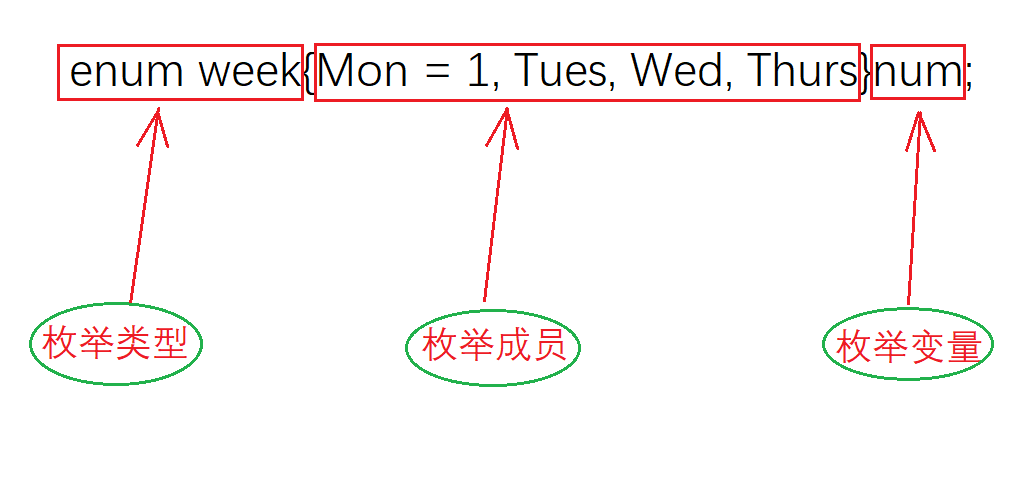
\includegraphics[scale = 0.3]{images/enum.png}
				\caption{枚举类型声明的结构体}
			\end{minipage}
		\end{figure}\par
		当枚举类型和枚举变量放在一起定义时,枚举类型的名字(就是enum week中的week)可以省略不写,枚举类型变量的赋值只能用自身的枚举成员来赋值,以上面的例子来说,num的赋值就只能用枚举成员Mon、Tues、Wed、Thurs,或者强制类型转换(enum week) 10,而不能用其他枚举类型的枚举成员来赋值。在显式赋值时,未指定的枚举名的值将依着最后一个指定值向后依次递增(注意是最后一个指定值),如下代码:\par
		\begin{lstlisting}
enum week{Mon = 1, Tues, Wed, Thurs, Fri = 10, Sat, Sun} num;
		\end{lstlisting}\par
		定义了一个枚举类型变量 \verb|num|,其实际绑定结果为:\verb|1, 2, 3, 4, 10, 11, 12|\par
		一个整数不能直接赋值给一个枚举变量,必须用该枚举变量所属的枚举类型进行类型强制转换后才能赋值,如\newline \verb|num = (enum week) 10|\par
		总结一下:
		\begin{enumerate}
			\item 在没有显示说明的情况下,枚举常量(也就是花括号中的常量名)默认第一个枚举常量的值为0,往后每个枚举常量依次递增1
			\item 在部分显示说明的情况下,未指定的枚举名的值将依着之前最有一个指定值向后依次递增
			\item 一个整数不能直接赋值给一个枚举变量,必须用该枚举变量所属的枚举类型进行类型强制转换后才能赋值
			\item 同一枚举类型中不同的枚举成员可以具有相同的值
			\item 同一个程序中不能定义同名的枚举类型,不同的枚举类型中也不能存在同名的枚举成员(枚举常量)
		\end{enumerate}
	\section{递归}
		递归就是\dots 套娃,还有一种DFS的味道

	\chapter{一些可能会用到的方法}
	\section{填充数组}
		当然,数组可以是动态分配也可以是直接分配。写题(尤其是答卷子)一般不需要考虑能开多大的数组
		\begin{enumerate}
			\item \verb|sprintf()| 函数,可以将输出的数据存进一个数组buffer里面
			\item \verb|memset()| 可以初始化一片连续的逻辑空间为0
			\item 有的时候可以采用 \verb|enum| 来代替数组,枚举类型类似于verilog的\verb|locoparam|,赋值可以\verb|int a = Mon|,但实际上a的值是1(如果周日是枚举表的第一个的话)
		\end{enumerate}
	\section{读入多组数据}
		可用 \verb|while( cin.getline(szLine,210) )| 的方式判断数据是否读完。\newline\texttt{cin.getline} 读取一行,第一个参数是缓冲区地址;第二个参数是缓冲区大小,为了防止越界用的。缓冲区不够大,就自动截断。它会自动往缓冲区末尾添加 `\texttt{\textbackslash 0}'。
		\subsection{scanf与while的使用}
		\paragraph{第一种用法} \verb|while(scanf("%d",&n),n)|\par
			功能:当n为0时中止循环\par
			这里要先说一下逗号表达式:逗号表达式的值是逗号后面的那个数。例如 \verb|x = (5,6)|,则 \verb|x == 6|。\verb|while(scanf("%d",&n),n)| 括号里的语句其实就是个逗号表达式,它的返回值是n的值,所以这个语句就相当于 \verb|while(n)|,\verb|n == 0| 时跳出循环,写成这样是为了同时输入。如果是 \verb|while( scanf("%d%d", &n, &m,), n, m )|,那么就相当于 \verb|while(m)|。
		\paragraph{第二种用法} \verb|while(scanf("%d", &n) != EOF)| 和 \verb|while(~scanf("%d", &n))|\par
			功能:当读到文件结尾时中止循环\par
			\verb|scanf| 语句的返回值为成功赋值的个数,例如 \verb|scanf("%d %d", &a, &b)|,如果a、b均赋值成功返回值为2,只是a赋值成功返回1,a、b都不成功返回0,出错的时候返回EOF。\verb|~| 是按位取反,scanf语句如果没有输入值就是返回-1,按位取反结果为0。\par
			注意:这两种方法在输入字母的时候会变成死循环,而 \verb|scanf("%d %d",&a,&b) == 2| 不会。windows下可通过按Ctrl +Z 并回车、linux下可通过 Ctrl + D 来达到“输入”文件结束符的效果,结束循环。
		\paragraph{第三种用法} \verb|while(scanf("%d",&n) == 1)|\par
			功能:赋值失败,跳出循环\par
			这个应该很好理解了吧,如果是 \verb|scanf("%d%d",&n,&m)| 就是\newline \verb|while(scanf("%d %d",&a,&b) == 2)|\par
			另外补充一下\textbf{取反}的用法:\verb|~| 是按位取反,由于计算机中数据存储为补码,故实际结果为$-x-1$。若是想要起到判0的作用,一个是使用 \verb|bool| 型变量,另一个也可以使用非 \verb|!|,如 \verb|!(2) == 0|
		\subsection{注意}
		在读取字符串存进数组的时候,可以直接用 \verb|cin| 直接整体读进去,但要注意在开数组的时候,要比字符串的最大长度\textbf{多1}!因为需要用来存 \verb|\0|
	\section{特殊运算}
		灵活利用位运算和求余运算,可以简化数值处理的过程。字符型数据同样可以按照ASCII码来计算(小写字母 = 大写字母 + 32)
	\section{一些语句}
		对于 \verb|if...else|,如果是多个if语句并列出现,则相当于是顺序的判断,当判断为假时不执行操作。而如果改成 if\dots else if\dots ,那么就具有了优先级的区分,当高优先级执行时就不会执行低优先级的语句了。
	\section{读入C风格的字符串}
		\verb|scanf("%s %s", array_a, array_b)| 注意这里没有 \verb|&|,因为数组名已经是入口地址了。或者用 \verb|cin>>array_a>>array_b| 也可以的

	\chapter{记录一些坑}
	\section{ends}
		\verb|ends| 不是想象中(老师讲的)那个输出一个高逼格的空格,它实际上是在缓冲区写入一个 \verb|'\0'|。对于Windows系统下,它会自己在输出的时候在 \verb|'\0'| 的位置加一个空格,但是Linux和macOS就什么都没有
	\section{数组}
		数组开大一点、大一点、大一点……比如字符串是两位的就直接开到 \verb|char array[5]|
\end{document}

